% Scribe template is a combination of 16831 and 10725. Thanks to those TAs!
\documentclass[11pt]{article}
\usepackage{latexsym}
\usepackage{amsmath}
\usepackage{amssymb}
\usepackage{amsthm}
\usepackage{bm}
\usepackage{epsfig}
\usepackage{listings}
\usepackage[tight]{subfigure}


\newcommand{\handout}[6]{
  \noindent
  \begin{center}
  \framebox{
    \vbox{
      \hbox to 5.78in { {#1} \hfill #2 }
      \vspace{4mm}
      \hbox to 5.78in { {\Large \hfill #6  \hfill} }
      \vspace{1mm}
      \hbox to 5.78in { {\em \hfill #3 \hfill} }
            \vspace{1mm}
      \hbox to 5.78in { {\em #4 \hfill #5} }
    }
  }
  \end{center}
  \vspace*{-1mm}
}

\newcommand{\lecture}[6]{\handout{#1}{#2}{#3}{#4}{#5}{#6}}

\newtheorem{theorem}{Theorem}
\newtheorem{corollary}[theorem]{Corollary}
\newtheorem{lemma}[theorem]{Lemma}
\newtheorem{observation}[theorem]{Observation}
\newtheorem{proposition}[theorem]{Proposition}
\newtheorem{definition}[theorem]{Definition}
\newtheorem{claim}[theorem]{Claim}
\newtheorem{fact}[theorem]{Fact}
\newtheorem{assumption}[theorem]{Assumption}

% 1-inch margins, from fullpage.sty by H.Partl, Version 2, Dec. 15, 1988.
\topmargin 0pt
\advance \topmargin by -\headheight
\advance \topmargin by -\headsep
\textheight 8.9in
\oddsidemargin 0pt
\evensidemargin \oddsidemargin
\marginparwidth 0.5in
\textwidth 6.5in

\parindent 0in
%\parskip 1.5ex
%\renewcommand{\baselinestretch}{1.25}

\begin{document}
\newcommand{\defeq}[0]{\ensuremath{\stackrel{\triangle}{=}}}
\def\x{\mathbf{x}}
\def\w{\mathbf{w}}
\def\K{\mathbf{K}}
\lecture{{\bf 16-822}: Geometry-based Methods in Vision (F18) }{Lecture \#0 \today}{Lecturer: Martial Hebert}{TA: Xiaofang Wang \& Xinshuo Weng}{Scribes: Scribe-1 \& Scribe-2$^1$}{\LaTeX~instructions}
\let\thefootnote\relax\footnotetext{$^1$ Your name, and Andrew-ID}





\section{Recap}
\begin{figure}[!h]
\begin{center}
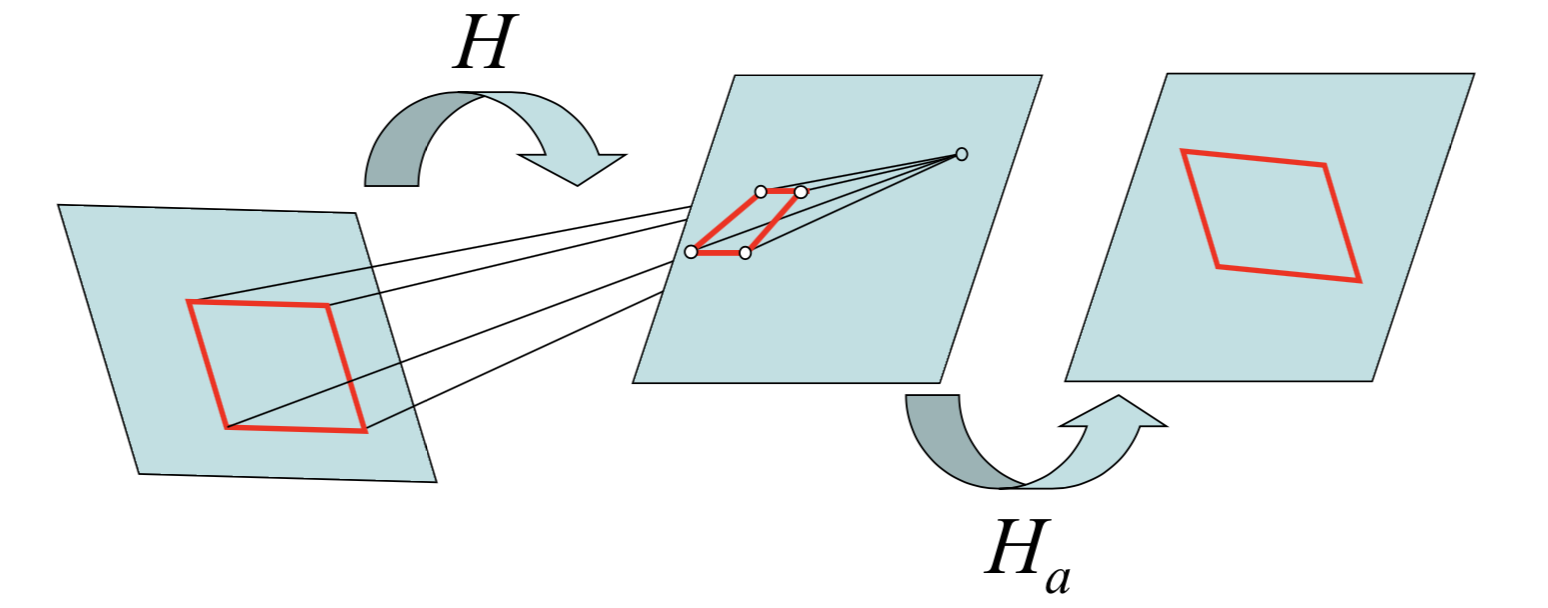
\includegraphics[width=10 cm]{images/affine_rect.png}
\caption{Affine planar rectification}
\label{affine_rect}
\end{center}
\end{figure}
Given a projective version of the world scene, as shown in Fig. \ref{affine_rect}, we may find a homography $H_a$ that preserves the parallelism and thus recovers affine properties as in the original plane. So $H_aH$ is an affine transformation. Actually, $H_a$ can be computed if we know the projection of the line at infinity. In this case, we may denote $l_\infty=\left[\begin{array}{ccc}l_1 & l_2 & l_3\end{array}\right]^\top$. $H_a$ can be expressed as
\begin{align*}
H_a = \left[
\begin{array}{ccc}
1 & 0 & 0 \\
0 & 1 & 0 \\
l_1 & l_2 & l_3
\end{array}\right]
\end{align*}





\section{Metric rectification}

\begin{figure}[!h]
\begin{center}
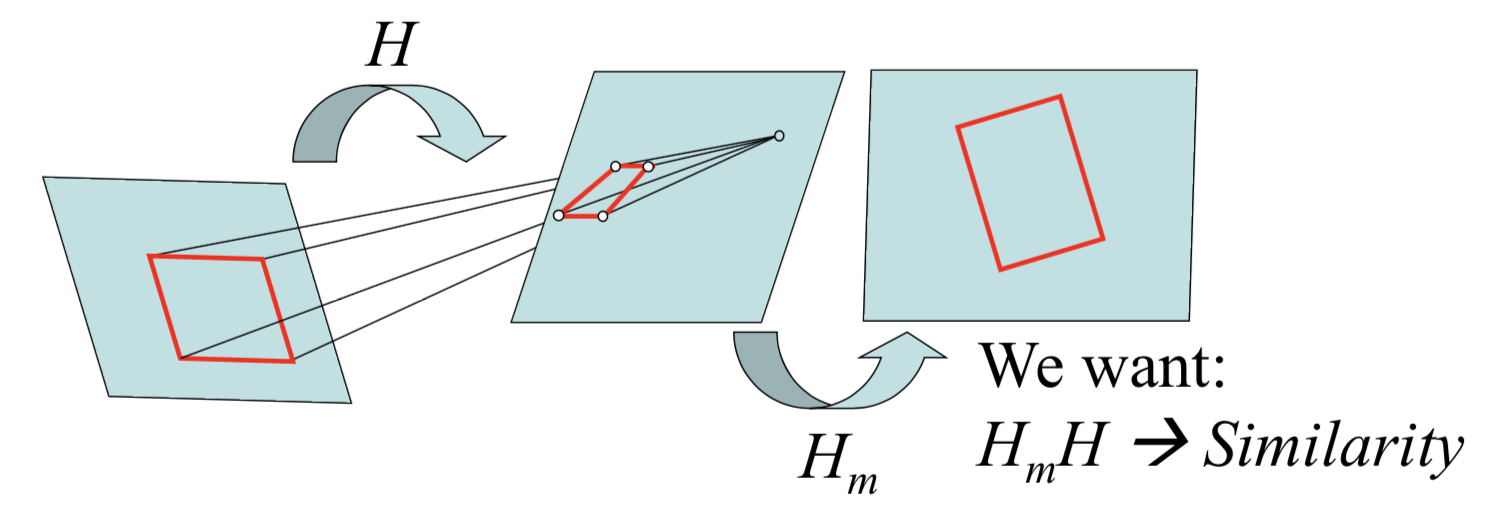
\includegraphics[width=10 cm]{images/metric_rect.png}
\caption{Metric planar rectification}
\label{metric_rect}
\end{center}
\end{figure}
Similarly, for metric rectification, the euclidean properties of the original plane can be recovered if we find a homography $H_m$, which preserves the angle between two lines on the plane.
We first denote two lines $l=\left[\begin{array}{ccc}a & b & c\end{array}\right]^\top$ and $l'=\left[\begin{array}{ccc}a' & b' & c'\end{array}\right]^\top$. The angle between these two lines is
\begin{align*}
\cos\theta = \frac{aa'+bb'}{\sqrt{a^2+b^2}\sqrt{a'^2+b'^2}}
\end{align*}
Given $aa'+bb'=l'^\top C^\ast l$ and $C^\ast=\left[
      \begin{array}{ccc}
       1 & 0 & 0 \\
       0 & 1 & 0 \\
       0 & 0 & 0 \\
      \end{array}
\right]$, we may derive that
\begin{align*}
\cos\theta = \frac{l'^\top C^\ast l}{\sqrt{l^\top C^\ast l}\sqrt{l'^\top C^\ast l'}}
\end{align*}
If $l'$ and $l$ are orthogonal, we have 
\begin{align*}
l'^\top C^\ast l = 0
\end{align*}

In Fig. \ref{metric_rect}, assume we have a line $l_0$ in the original plane and its homography transformation $l$. After metric rectification, the line became $l'$ and right angle preserved. We get the following equation
\begin{align*}
l'=H^{-\top}_mH^{-\top}l_0=H^{-\top}l \\
l
\end{align*}












\end{document}
